\documentclass[cm, 10pt]{article}
% =================================================================== %
%                                                                     %
% Packages                              %
%                                                                     %
% =================================================================== %

% For adjusting the page dimensions to look passable instead of
% terrible
\usepackage[margin=1in,tmargin=1.25in,paper=letterpaper]{geometry}

% For most of the math symbols, and nice things like align
% environment
\usepackage{amsmath, amssymb, mathtools}

% For linking content outside of the document
\usepackage{hyperref}

% Fancy page header
\usepackage{fancyhdr}

% For customizing the enumerate environment
\usepackage{enumitem}

% For diagrams, if needed
\usepackage{tikz}
\usepackage{pgfplots}
\usetikzlibrary{positioning}

\usepackage{courier}

% For figure
\usepackage{float}

% For the page of... in footer
\usepackage{lastpage}

% For cancelling frac stuff
\usepackage{cancel}

\usepackage{titlesec}

% ----------------------- Hacky Control Seqs ------------------------ %
\let\oldref\ref
\renewcommand{\ref}[1]{(\oldref{#1})}

\newcommand\RR{{\mathbb R}}
\newcommand\CC{{\mathbb C}}
\newcommand\ZZ{{\mathbb Z}}
\newcommand\NN{{\mathbb N}}
\newcommand\QQ{{\mathbb Q}}

\newcommand{\set}[1]{\ensuremath{ \left\{ #1 \right\} }}
\newcommand{\pn}[1]{\left( #1 \right)}
\newcommand{\abs}[1]{\left| #1 \right|}
\newcommand{\bk}[1]{\left[ #1 \right]}
\newcommand{\vc}[1]{\left\langle #1 \right\rangle}

\newcommand{\dd}{\mathrm{d}}
\newcommand{\LL}{\mathcal{L}}

\newcommand{\st}{\text{ st }}
% ----------------- pset specific control sequences ----------------- %
\newcommand{\ucf}{U_{\rm cf}}
\newcommand{\ueff}{U_{\rm eff}}

\newcommand{\rmax}{r_{\rm max}}
\newcommand{\rmin}{r_{\rm min}}

\renewcommand{\vec}[1]{\mathbf{#1}}

% Finally, enumerate formatting
\setenumerate[0]{label=(\alph*)}

% And shorten the vspace after section headers. How to read?
%
%                {12pt plus 4pt minus 2pt}
%
%  - 12pt is what we would like the spacing to be
%  - plus 4pt means that TeX can stretch it by at most 4pt
%  - minus 2pt means that TeX can shrink it by at most 2pt

\titlespacing\section{0pt}{
  12pt plus 2pt minus 2pt}{
  0pt plus 2pt minus 2pt}

% ----------------------- Header formatting ------------------------- %
\pagestyle{fancy}
\fancyhf{}
\lhead{Forest Kobayashi, Harry Fetsch}
\chead{Computational Project}
\rhead{Phyiscs 111 - Fall \the\year}
\lfoot{Due Sunday, December 10th}
\rfoot{\thepage\ of \pageref{LastPage}}

% Adjust paragraph formatting
\setlength{\parindent}{0pt}
\setlength{\parskip}{1em}

% Finally, enumerate formatting
\setenumerate[0]{label=(\alph*)}

% ================================================================== %
%                                                                    %
% Document                              %
%                                                                    %
% ================================================================== %

\begin{document}

\section{Introduction}
For our computational project, we chose to investigate the
$n$-body problem. As we showed in class, this system is not
analytically solvable, so our investigation centers on simulating
these masses’ interactions efficiently so that we can see how the
system evolves based on various initial configurations. Solving
n-body problems has applications in modeling celestial phenomena,
and as a natural extension of the same techniques, other forces
could be calculated to model the behavior of gases.
\subsection{The Algorithm}
For our simulation, we employed the Barnes-Hut algorithm, a
tree-based approximation scheme that drops asymptotic
computational complexity from $O\pn{n^2}$ to $O\pn{n\log{n}}$
with negligible degradation in accuracy. Our particular
implementation can be broken down into the following steps:
\begin{enumerate}
  \item First, we initialize the masses as follows:
    \begin{enumerate}[label=\roman*)]
      \item We randomly select the magnitude of mass's displacement
        from the origin of the space (denoted $r$) from one of three
        distributions:
        \begin{enumerate}[label=\arabic*.]
          \item A simple linear distribution (uniform range between
            some start and stop points $r_a$ and $r_b$)
          \item A normal distribution, characterized by a mean radius
            $\overline{r}$ and a standard deviation $\sigma$, yielding
            a probability density function of
            \[
              \frac{1}{\sqrt{2 \pi \sigma^2}}e^{-\frac{(x -
                  \overline{r})^2}{2\sigma^2}}
            \]
          \item A gamma distribution, characterized by two parameters:
            the ``shape'', $k$ and, ``scale'', $\theta$, yielding a
            probability density function of
            \[
              f(x; k,\theta) = \frac{x^{k-1}e^{-x/\theta}}{\theta^k
                \Gamma(k)}
            \]
            (where $\Gamma(k)$ is the gamma function. Source:
            \emph{Gamma Distribution}, Paul E. Johnson).
          \end{enumerate}
        \item Next, we choose a second set of distributions (of the
          three above) from which to sample $\phi_1, \phi_2, \ldots,
          \phi_{n-1}$, to express the point in $n$-D spherical
          coordinates. We then projected the points back into $\RR^n$,
          using the following formulae:
          \begin{align*}
            x_1 &= r\cos(\phi_1) \\
            x_2 &= r\sin(\phi_1)\cos(\phi_2) \\
            x_3 &= r\sin(\phi_1)\sin(\phi_2)\cos(\phi_3) \\
                &~\,\vdots \\
            x_{n-1} &= r\sin(\phi_1) \cdots \sin(\phi_{n-2}) \cos(\phi_{n-1}) \\
            x_n &= r\sin(\phi_1) \cdots \sin(\phi_{n-2})\sin(\phi_{n-1})
          \end{align*}
          Where $\forall i \in \NN \st 1 \leq i \leq n-2, \phi_i \in
          \bk{0,\pi}$, while for $i = n-1$, we have $\phi_i \in \bk{0,
            2\pi}$.
        \item Repeat i) for velocities, but only use a linear
          distributions for theta in ii) (we want our velocities to
          show no bias in direction, so that for large numbers of
          particles, the total momentum of the system will be
          approximately 0. Since all the thetas are simple linear
          distributions, we'd expect approximately uniform
          distribution of $\hat{r} = \vec{r} / r$ for large values of
          $n$).\footnote{Note that for repeatability during our
            testing phase, we used consistent RNG seeds between runs
            for each of our generator functions, each of which was
            itself generated by a static-ly seeded function. However,
            the current algorithm uses OS-derived RNG to seed the
            distributions.}
        \item Next, we ingest the masses by pushing each generated
          body to a holding queue for the root node of our global tree
          structure.\footnote{In the actual codebase itself, it should
            be noted that each instance of our \texttt{Region} class
            (which stores the data for a single node on our tree) is
            wrapped in special layering classes, called \texttt{Arc}
            and \texttt{Mutex}. The data for the \texttt{Arc} class is
            stored in read-only memory, and contains a reference to
            the \texttt{Mutex} class, which further wraps pointers to
            the object with a guarding layer that locks out new
            threads when the memory is being modified. Thus, we can
            safely have multiple threads checking whether the Region
            is currently in use (by calling methods on the Mutex)
            without creating data races.} At this point,
          initialization is complete, and we proceed to the main
          algorithm.
  \end{enumerate}
\item First, the space is recursively subdivided into $2^n$ $n$-D
  subcubes of our overall simulation region (in the the 2-D case,
  these would be quadrants). Each sub-cube is subdivided further,
  until it contains either 0 or 1 masses, with an absolute limit on
  the minimum side-length of any region, which we store as a static
  float \texttt{MIN\_LEN} (a tiny fraction of our global simulation
  width). This data structure can be visualized as a large tree, in
  which each node has either 0 or $n$ child nodes.
  \begin{enumerate}[label=\roman*)]
    \item At this point, to save on computation, any remaining
      sub-bodies are merged into a single body at their center of
      mass, with momentum equal to the sum of their incident momenta.
      This have a negligible effect on any force-calculations, since
      the vast majority of mass interactions will occur on length
      scales orders of magnitude larger than \texttt{MIN\_LEN}.
  \end{enumerate}
\item Once the initial tree has been drawn, we recurse downwards until
  we reach a leaf node. If the node is empty, we return. Else, there
  must be only one body inside the region, and we begin calculating
  the net acceleration on it.
  \begin{enumerate}[label=\roman*)]
    \item To calculate the acceleration on a mass $m$, we start at the
      top of the tree, and compare the distance $m$ and the center of
      the smallest bounding region about $N$. We denote this distance
      by $d$. Let the side length of the bounding region on $N$ be
      denoted $s$. We define a ``distance`` metric, $\theta$, as
      follows:
      \[
        \theta = \frac{s}{d}
      \]
      If $\theta$ is greater than some specific threshold value, then
      we calculate the center of mass of $N$, and use Newton's Law of
      Gravitation on this center of mass to obtain a portion of the
      force on $m$. Note that this is a reasonable approximation
      because, for large distances, the gravitational field from a
      collection of masses becomes approximately the gravitational
      field from their center of mass.
    \item Else, If the current region is not far enough away to make
      this approximation, we check to see if it has child regions, or
      if it holds a mass (note that because each region has 0 or 1
      masses, these are mutually exclusive). If it has a mass, we
      calculate the acceleration because $N$ and that mass.
    \item If the current region instead has child regions, we
      recursively call the same update acceleration function on each
      of them. This will recurse until it finds a region with 1 mass,
      an empty region, or a region far enough away to approximate. It
      will then return back to the top of the tree, combining the
      results of every acceleration calculation to get one total
      acceleration for $N$
  \end{enumerate}
\end{enumerate}

\subsection{The System}
The simulation that we developed contains several masses, each of
which have (non-relativistic) velocities and positions in a space of
arbitrary dimensions. In order to obtain reasonably interpretable
results, we chose to generate our plots using a 2-dimensional space,
but there is abundant room for future study in analyzing the
interactions of bodies in higher dimensions.
\begin{enumerate}
  \item The system, when run in 2 dimensions, has $2n$ degrees of
    freedom: $x_1(t), x_2(t), \ldots, x_n(t)$, and $y_1(t), y_2(t),
    \ldots y_n(t)$. Each body also has a constant mass.
  \item The system depends on several dimensionless constants. These
    values are arbitrary, but we chose them with several factors in
    mind. \texttt{DT}, the timestep, needs to be large enough to
    obtain results in a reasonable amount of time, but small enough
    that the simulation is reasonably similar to the continuous
    real-time system. We chose \texttt{G} to be 16000 because this is
    easy to plug into equations to determine the initial conditions
    that generate simple trajectories (for example, a circular orbit,
    see below).
\end{enumerate}

% ------------------------------------------------------------------ %

\section{Analysis}
Because this setup is too general to study and get meaningful results,
we simulated several sets of initial conditions that have the
possibility of giving interesting behavior. These conditions include:
\begin{enumerate}
  \item A two-body gravitational simulation with identical masses.
    Because this is analytically tractable, this configuration is a
    good way of checking that the simulation gives accurate results.
    It also gives a way to analyze the error in the simulation caused
    by rounding and discrete time steps.
  \item A system with two large objects orbiting, and several smaller
    objects injected randomly around them, similarly to the three-body
    simulation showed in class. This simulates a binary star system,
    with a number of planets or other celestial bodies interacting
    with it. Some have bound orbits that eventually get close enough
    to the large bodies that they collide, and some have enough
    velocity to escape.
  \item A scattering problem, with two large orbiting masses in the
    center, and a large set of small masses injected from the side.
    This shares some elements in common with the binary system (b),
    and with the scattering calculations done in class.
\end{enumerate}

% ------------------------------------------------------------------ %

\section{Findings}
\begin{enumerate}
  \item Placing two bodies with positions and velocities that would
    generate a circular orbit in Newtonian physics lead (thankfully)
    to two the bodies orbiting their shared center of mass.

    As we can see, the shape of the orbit is circular with a very
    slight precession. This can be explained in part by the numerical
    rounding used by the programming language. In addition, the fact
    that discrete timesteps were used means that, instead of being a
    true circle, each body's orbit is composed of many linear steps
    that form a circular shape. This means that the bodies are not
    interacting continuously throughout their orbits, but only once
    every time step. Therefore, it is unsurprising that there is a
    small perturbation from the analytical solution, but as we can
    see, this is small enough that the simulation can still be used to
    give an excellent approximation of behavior.
    \begin{figure}[H]
      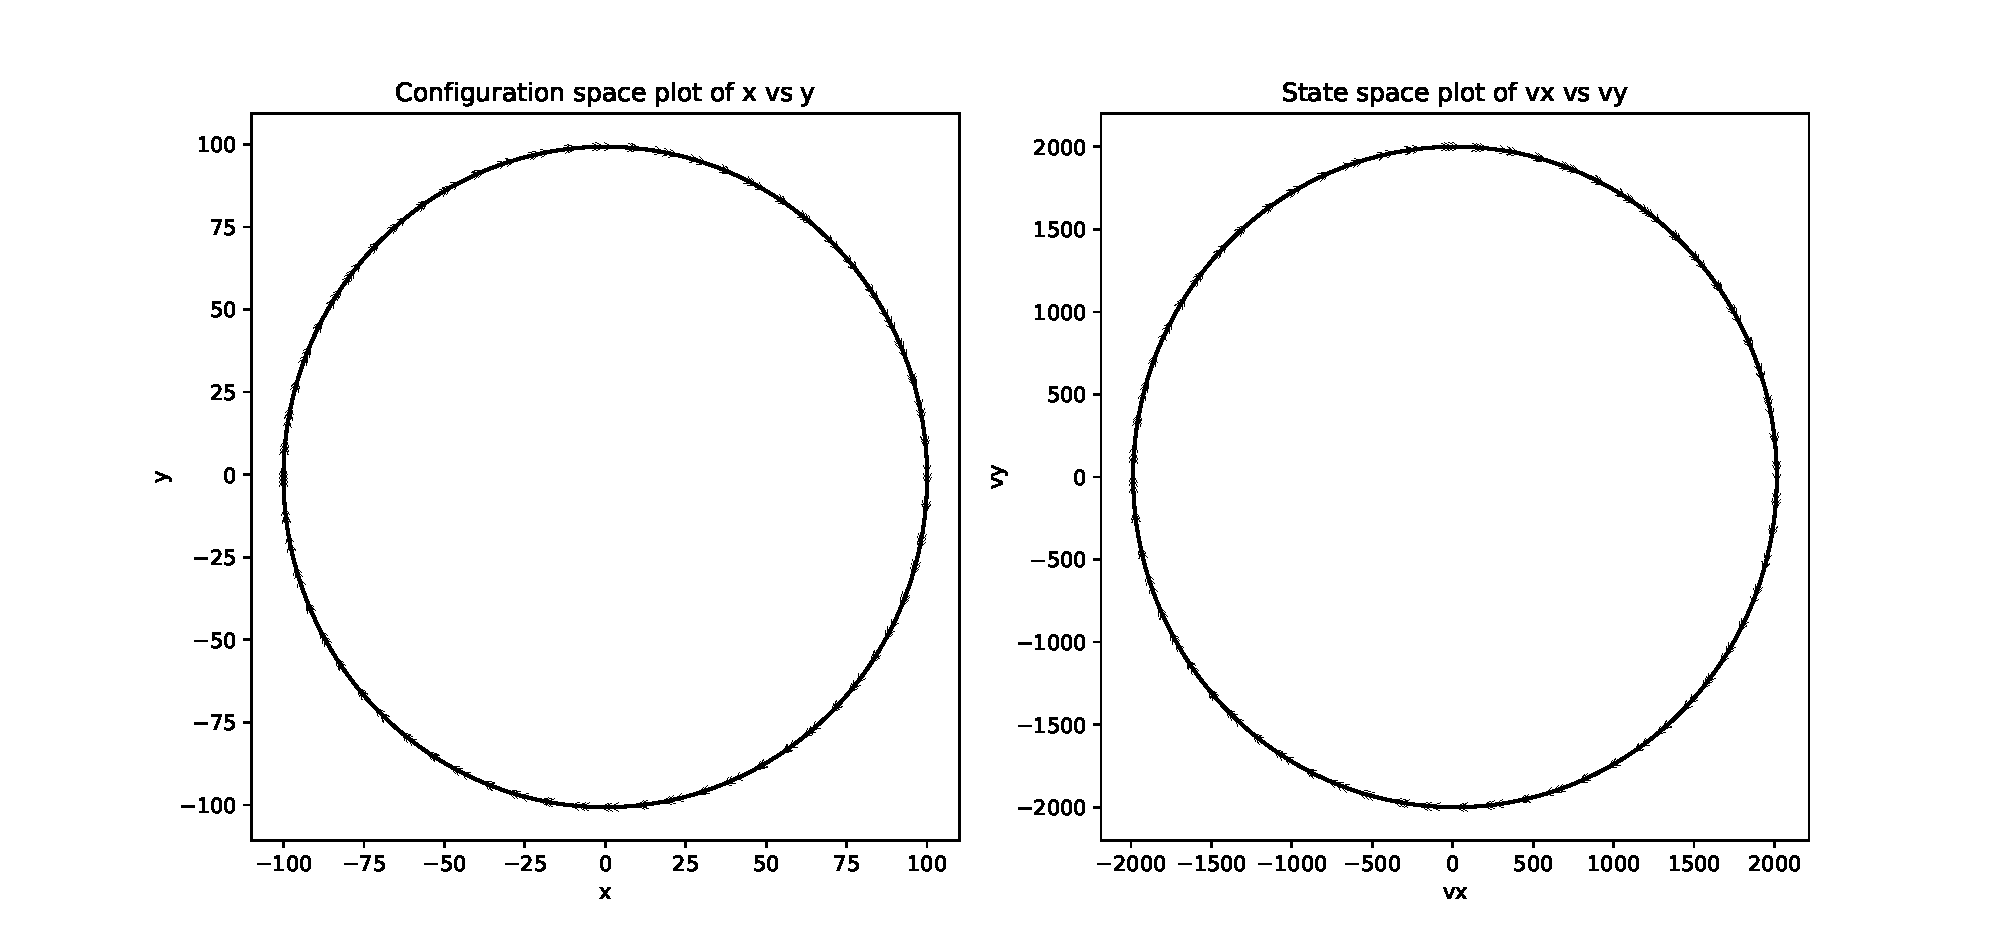
\includegraphics[width=\linewidth]{binary_config.pdf}
    \end{figure}
    \begin{figure}[H]
      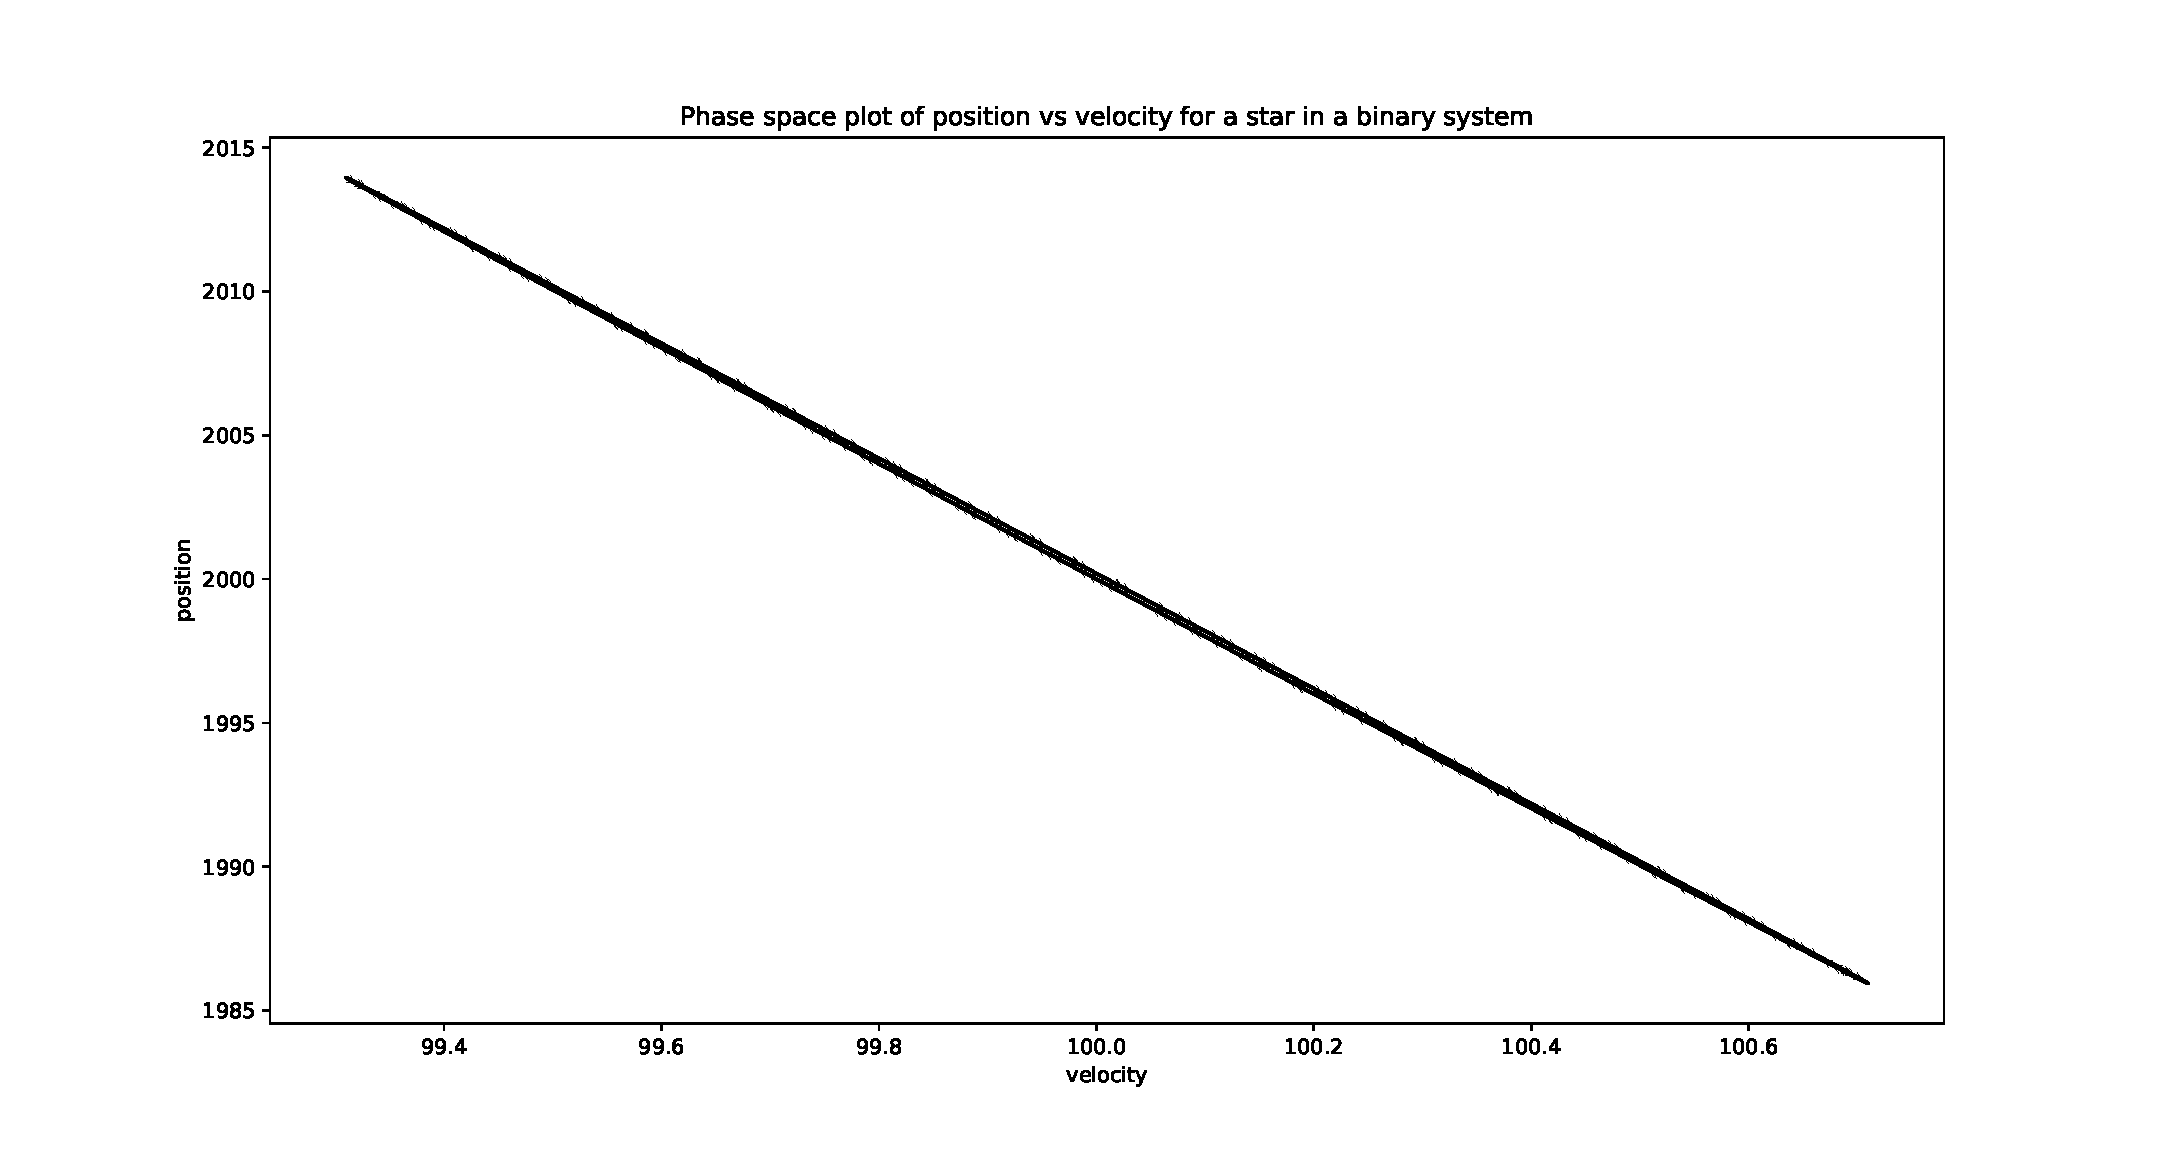
\includegraphics[width=\linewidth]{binary_phase.pdf}
    \end{figure}

  \item As shown in the attached video
    (\url{https://youtu.be/BcRRBVifNFI}), each of the masses injected
    into the binary system has slightly different initial conditions,
    but their final conditions are vastly different. Most are ejected
    from the simulation, some collide and are absorbed by the large
    masses, and a few continue to orbit in an unstable configuration
    around the large masses.
  \item We see again in the following plots that, even for small
    changes in initial conditions, bodies have completely different
    trajectories both in phase space and in configuration space.
    Because of the size limits of our simulation, we saw widely
    varying scattering results very every impact parameter that was
    tested. However, there is room for futher investigation by testing
    much higher impact parameters to find the ones for which bodies
    are negligibly scattered by the binary system.
    \newline
    The following plots track two masses injected from the left and
    scattering off of a system of two large bodies orbiting circularly
    about their barycenter.
    \begin{figure}[H]
      \centering
      \begin{minipage}{.49\linewidth}
        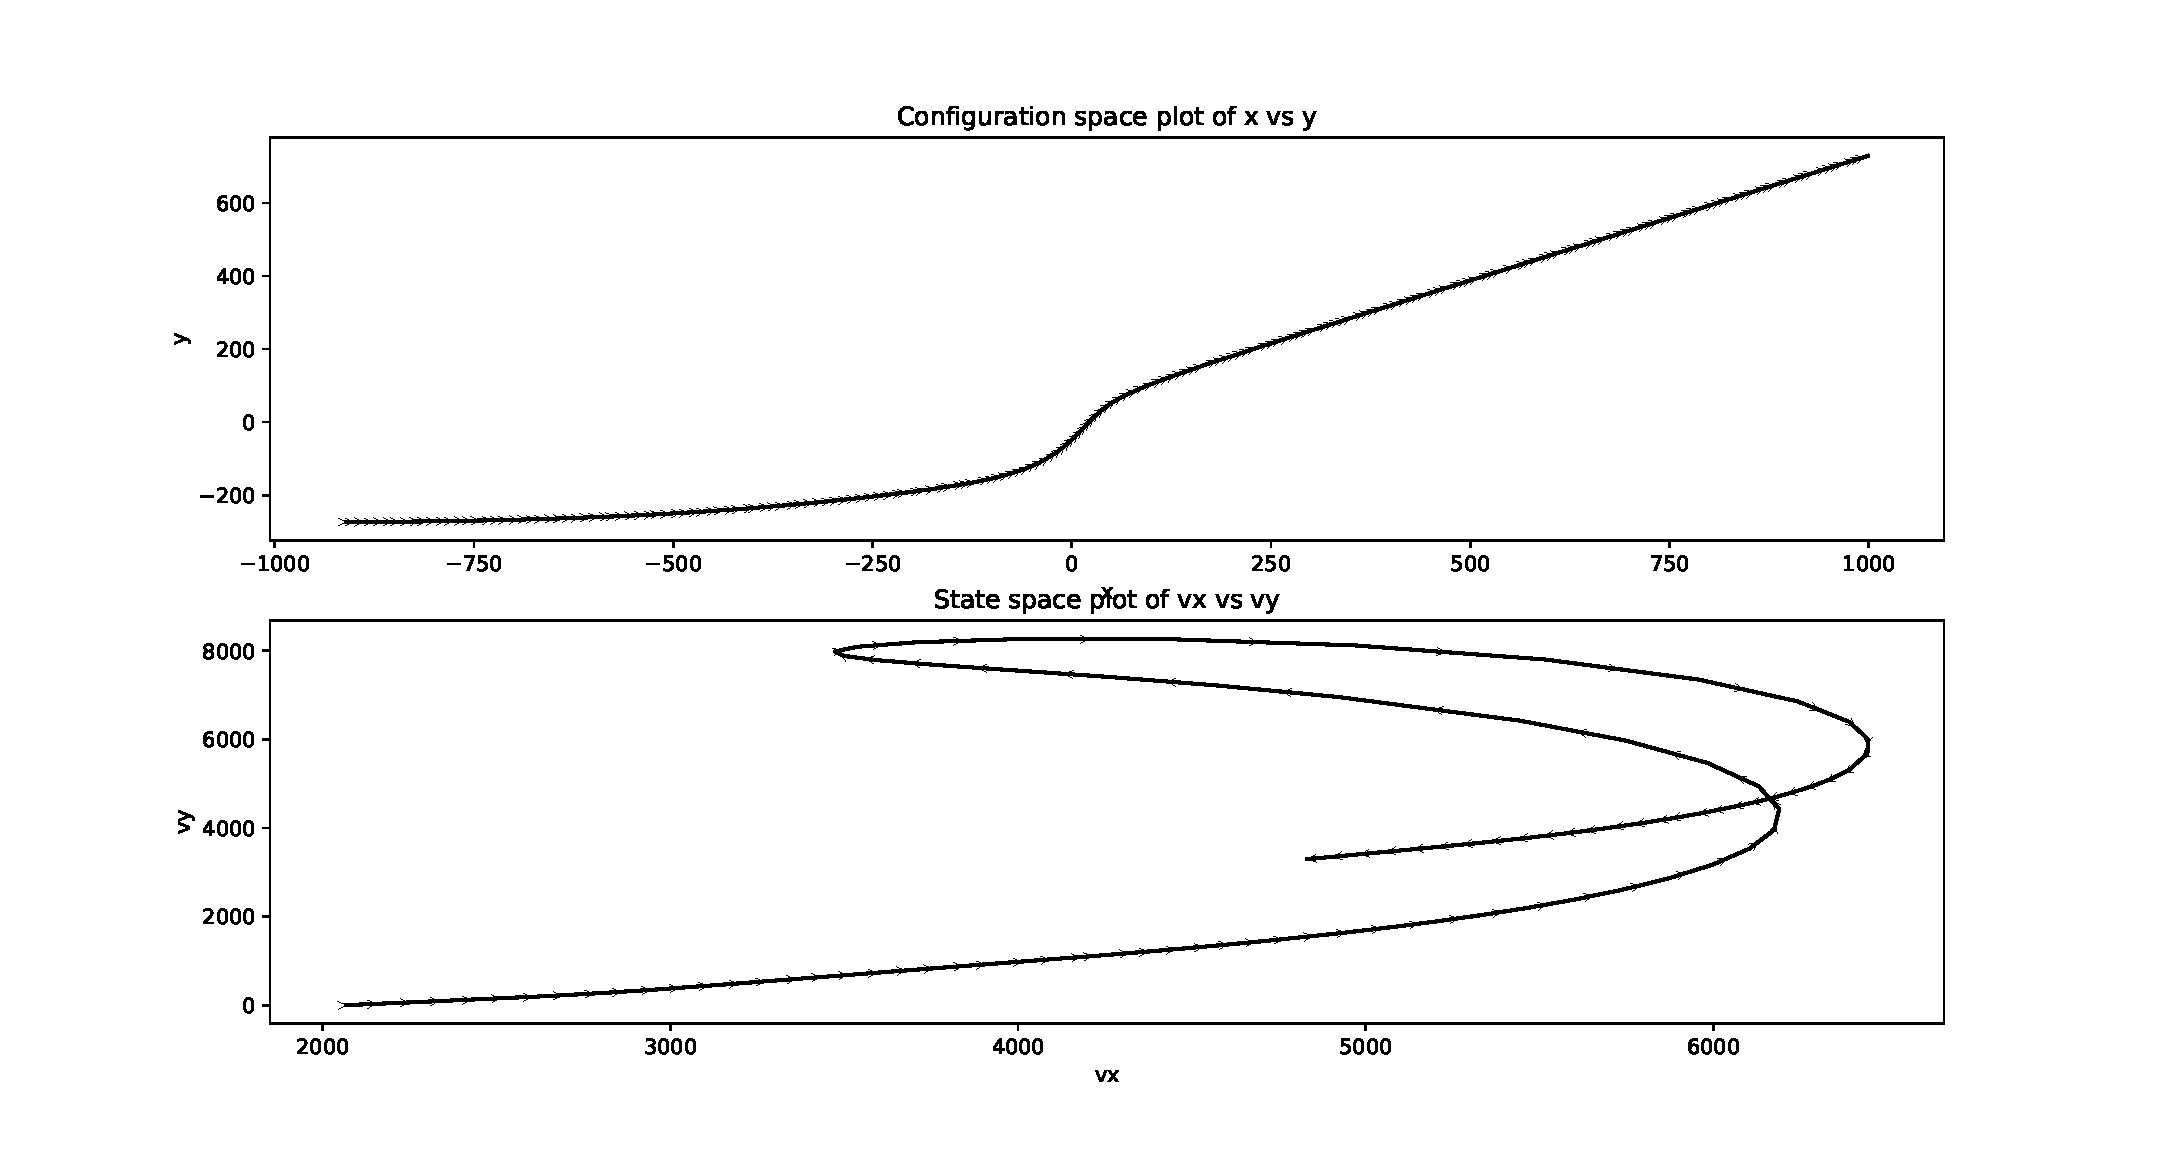
\includegraphics[width=\linewidth, height = 11cm]{m1space.pdf}
      \end{minipage}
      \begin{minipage}{.49\linewidth}
        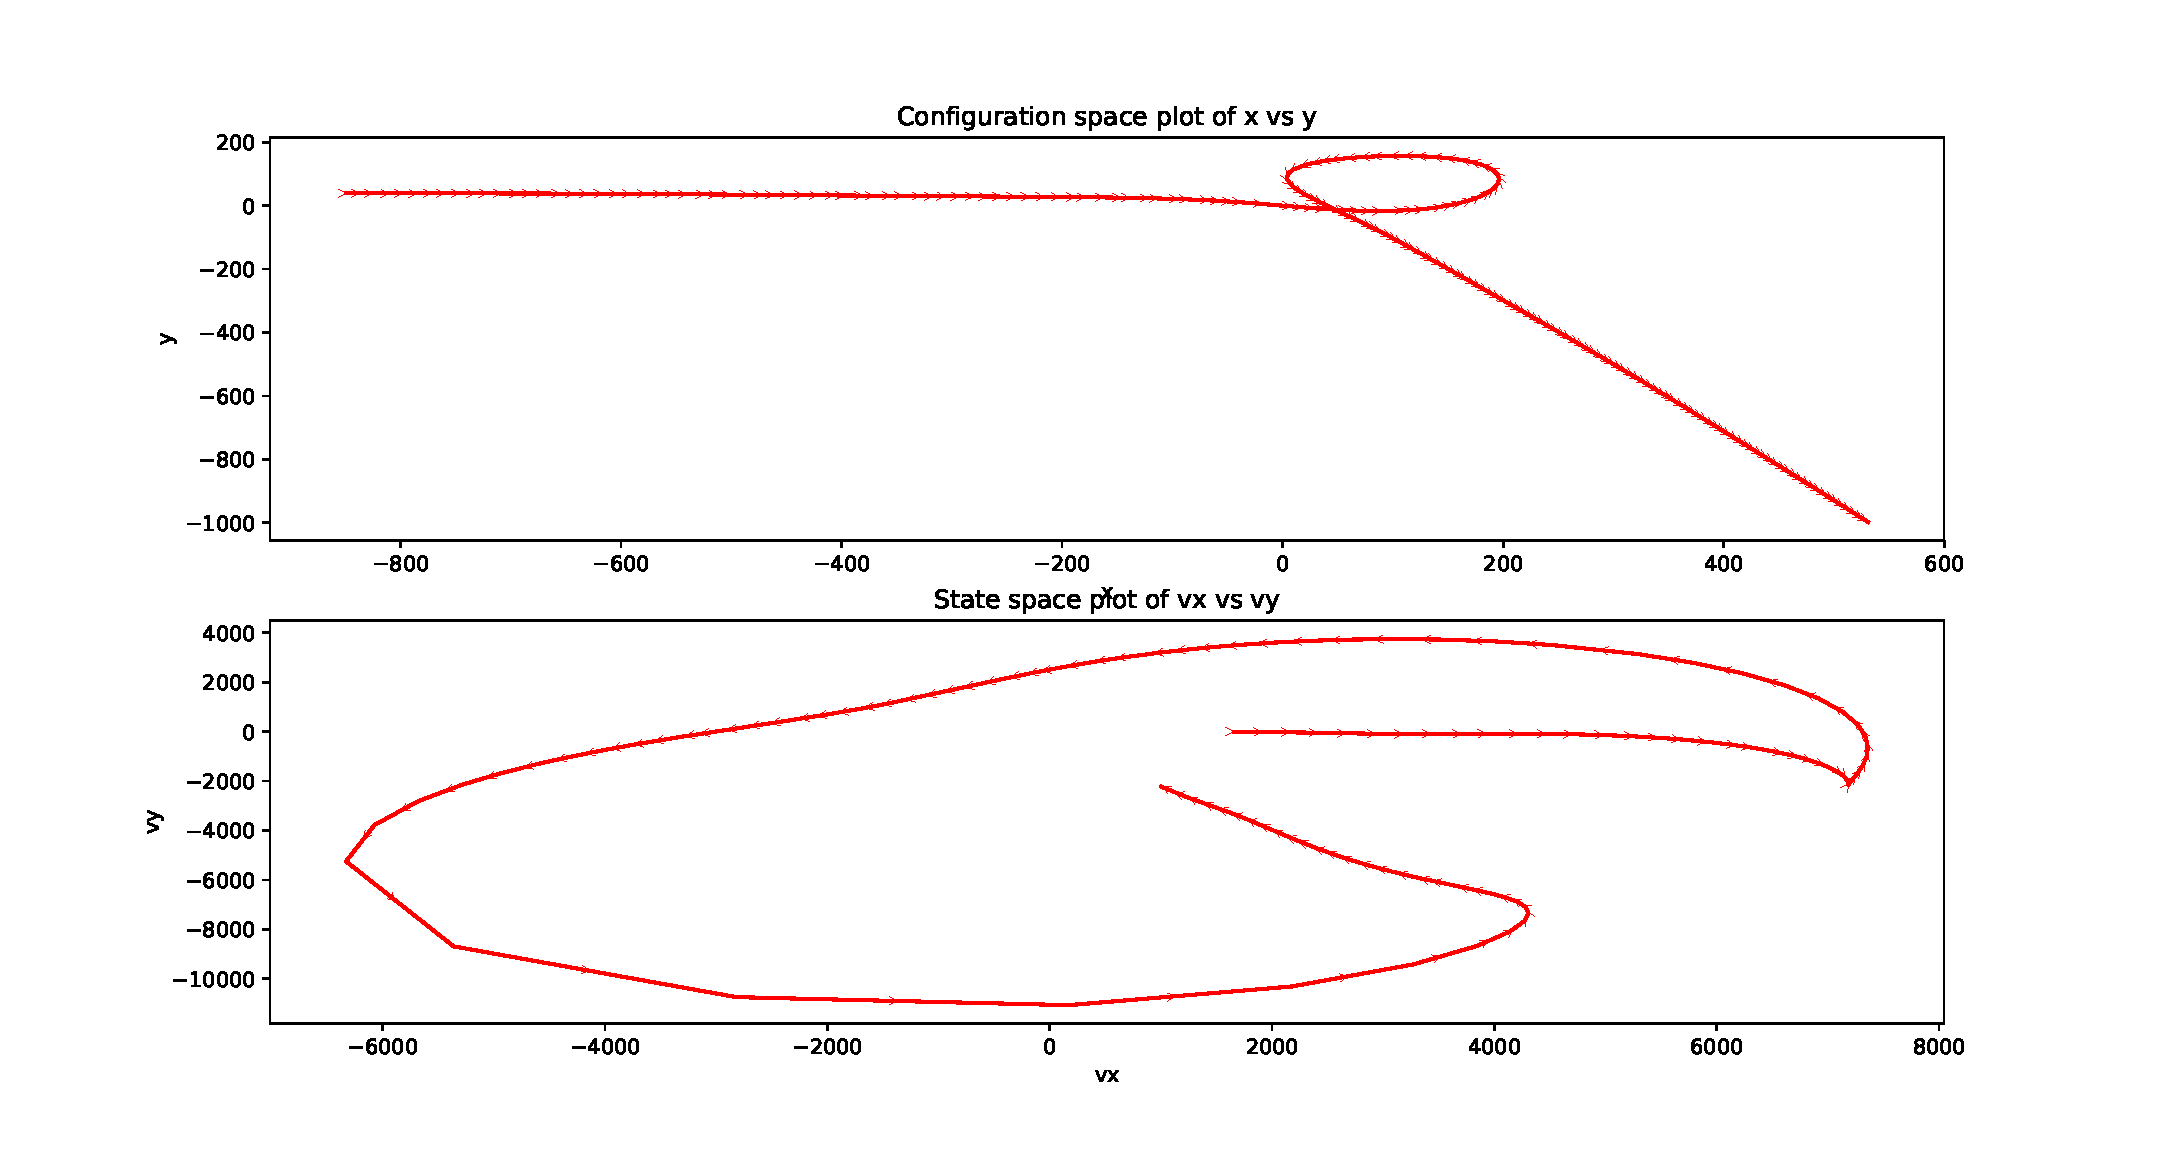
\includegraphics[width=\linewidth, height = 11cm]{m2space.pdf}
      \end{minipage}
    \end{figure}
    \begin{figure}[H]
      \centering
      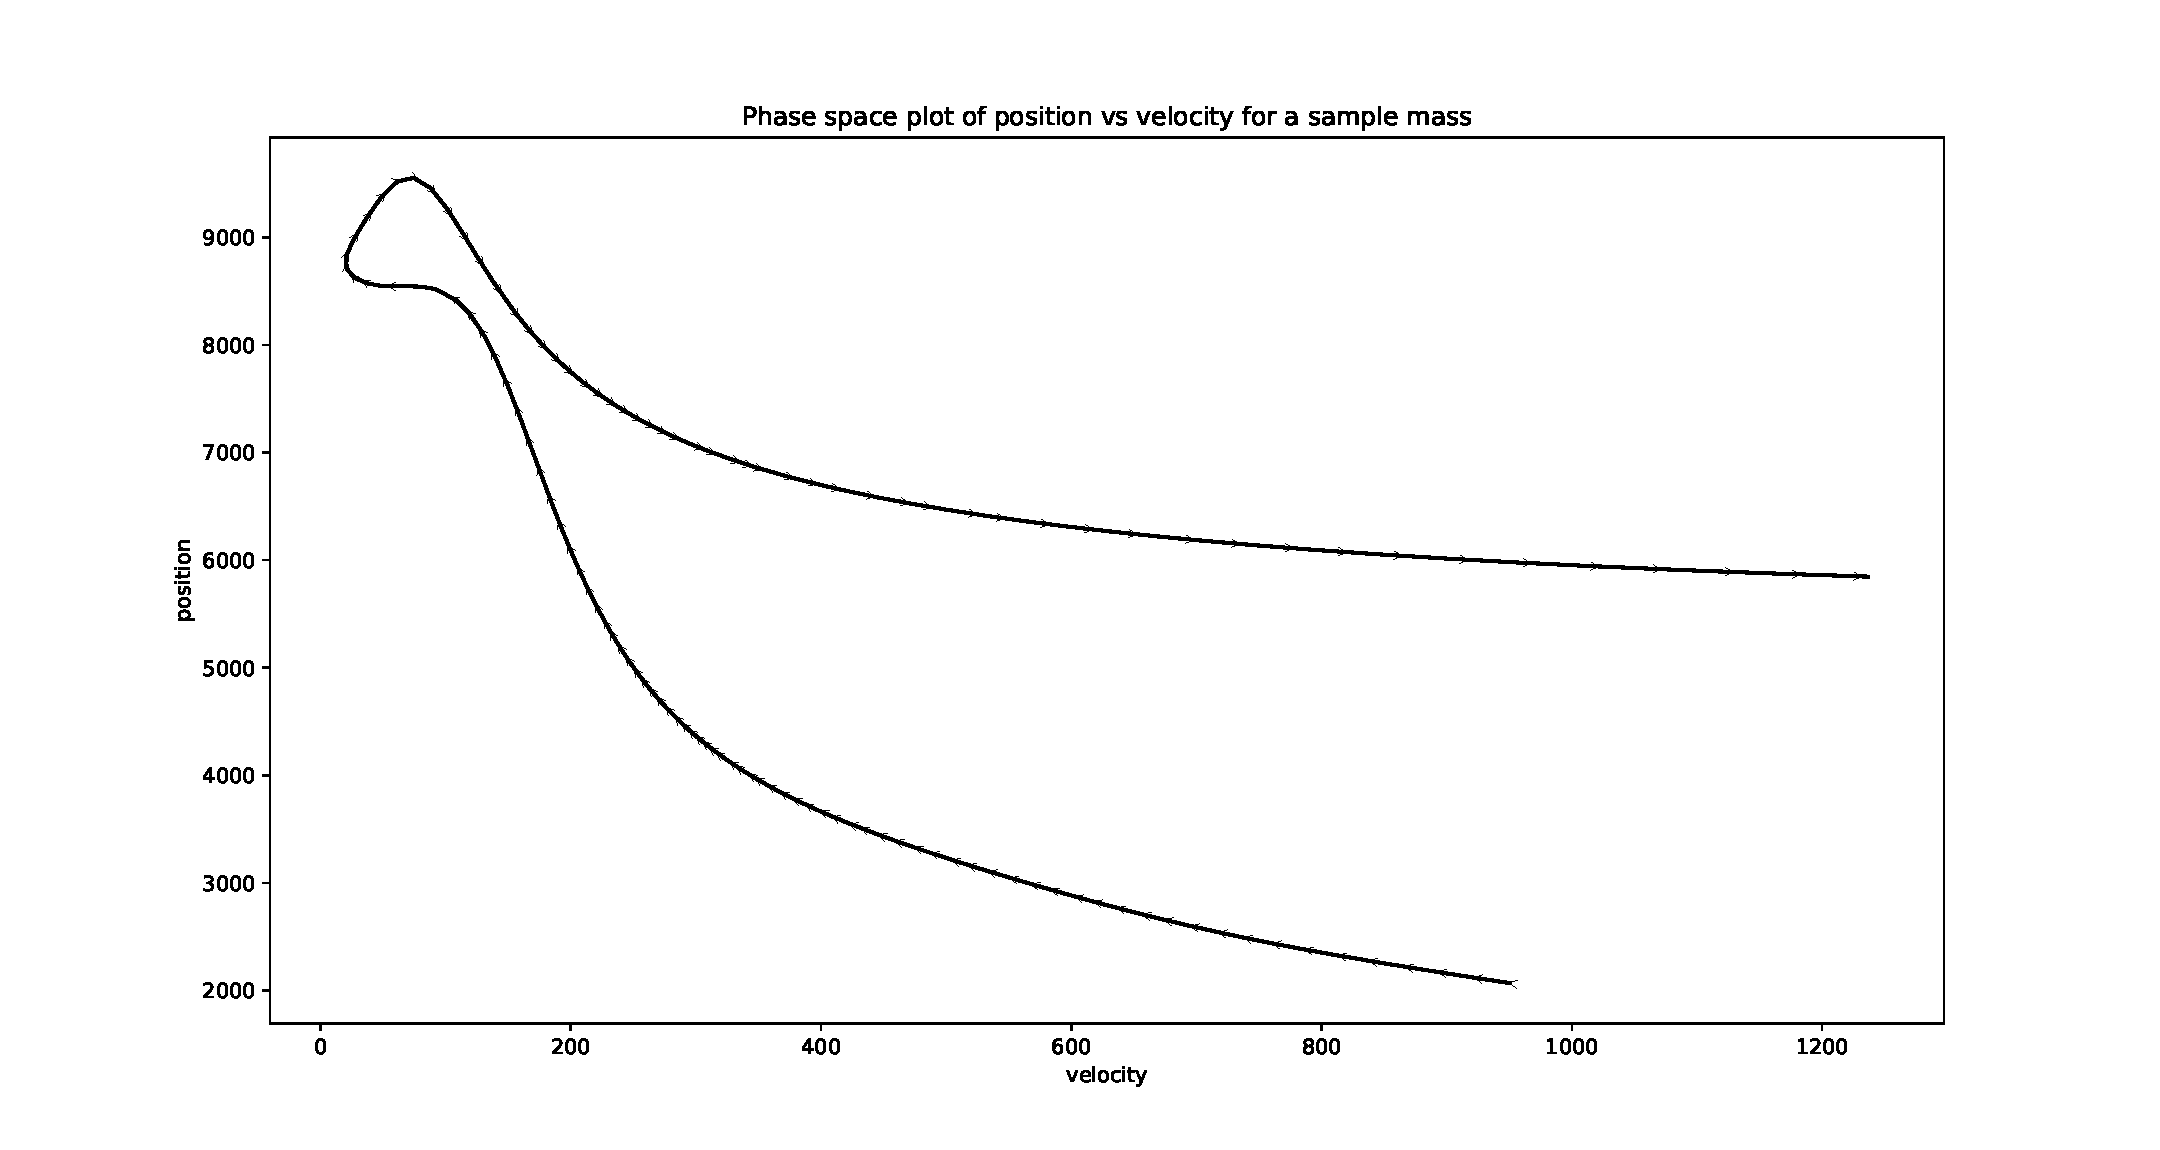
\includegraphics[width=\linewidth]{m1phase.pdf}
    \end{figure}
    \begin{figure}[H]
      \centering
      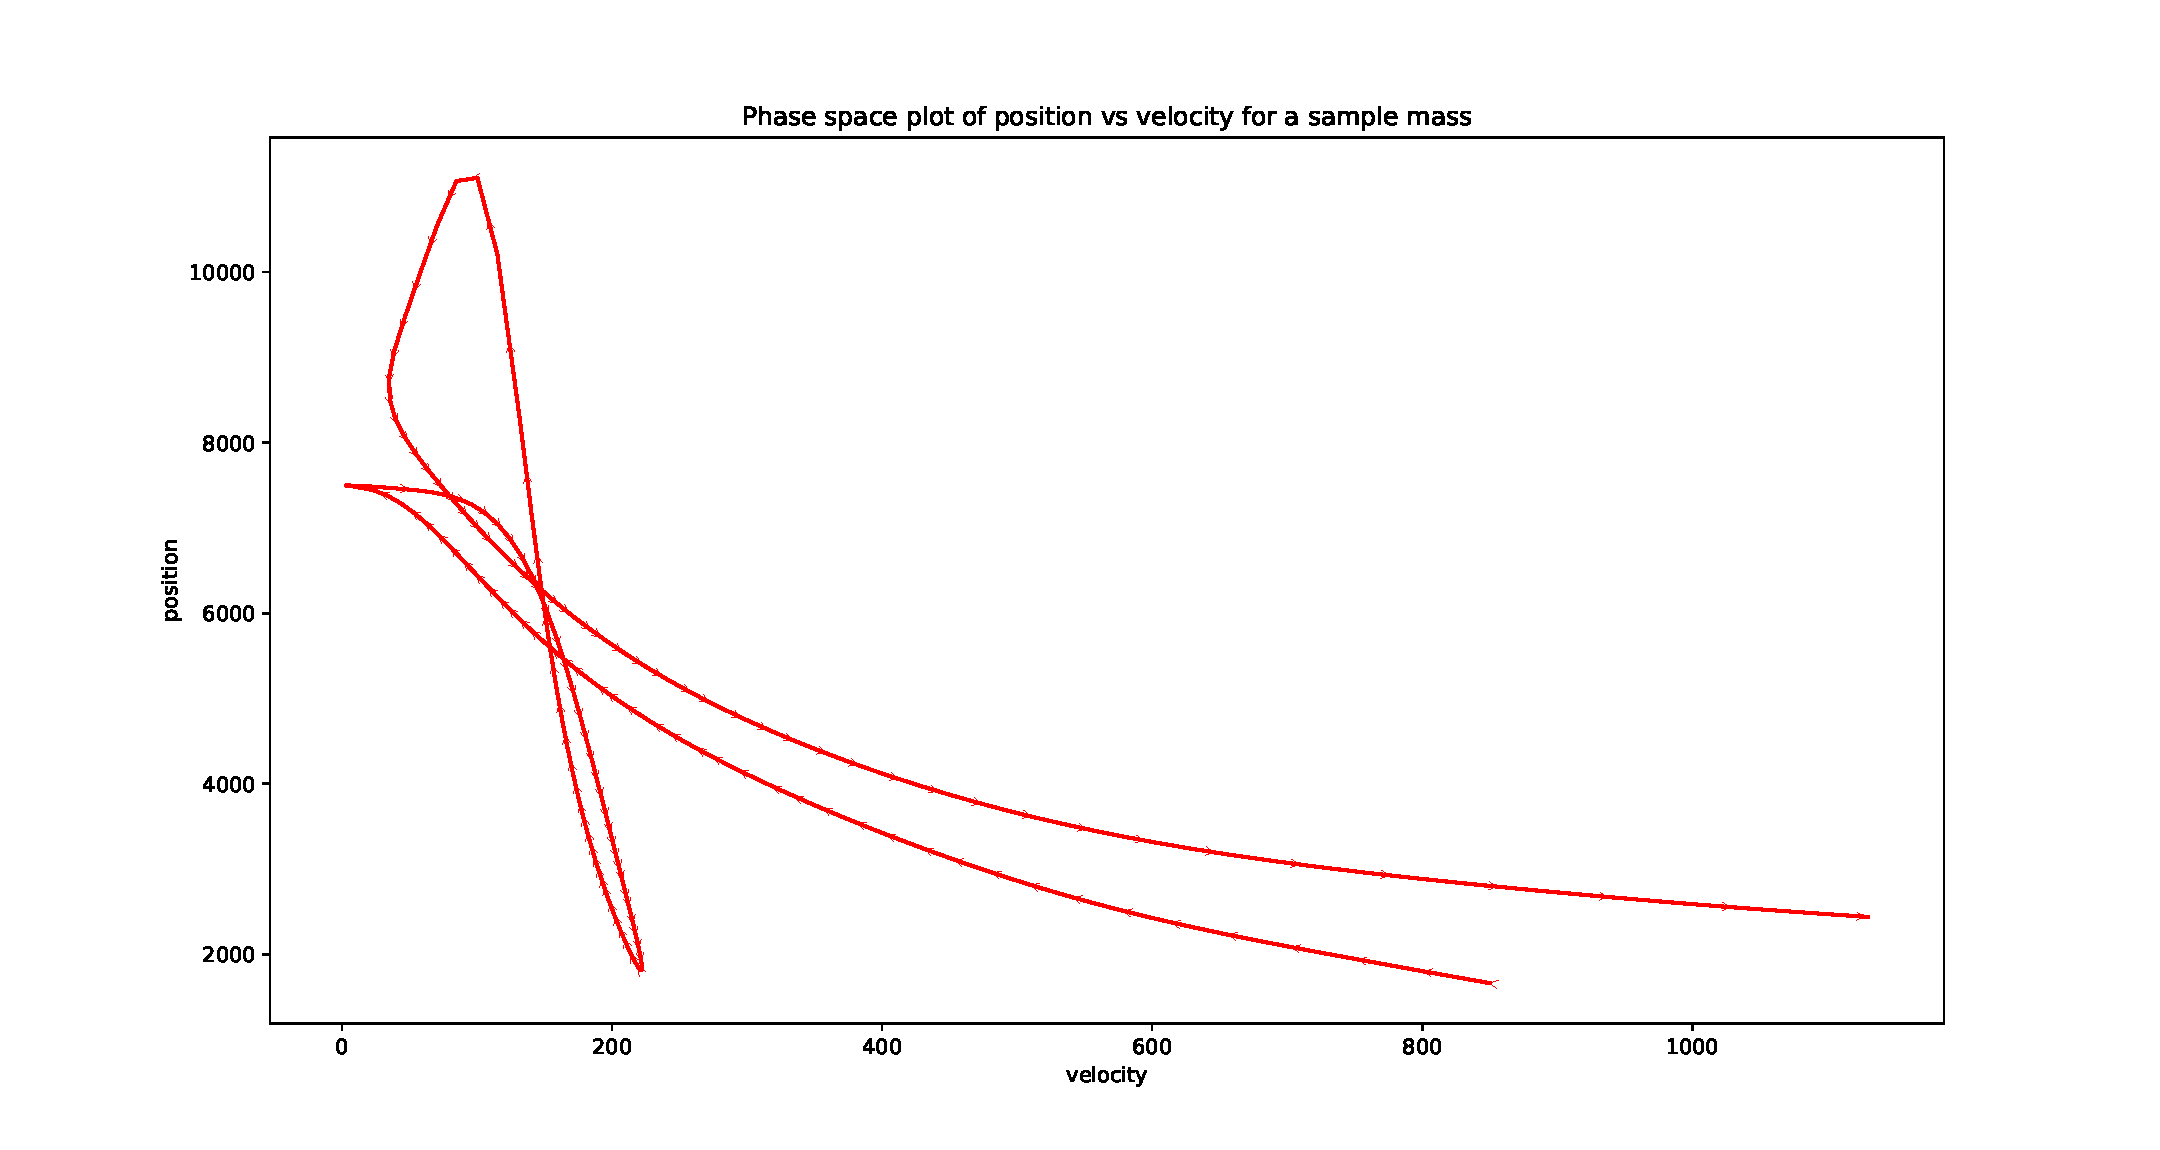
\includegraphics[width=\linewidth]{m2phase.pdf}
    \end{figure}
\end{enumerate}
% ------------------------------------------------------------------ %

\section{Conclusion}
The predominant theme in analyzing our findings for each system was
that final state differed significantly even for small changes in the
initial conditions. From this we conclude that our system is chaotic.
This is not at all surprising --- after all, the $n$-body problem is
known to be analytically intractable. We further conclude that,
although our simulation contains very small numerical errors due to
rounding and discrete time steps, these are small enough (and
accumulate slowly enough) that we can extract meaningful data about
real interactions from our simulation.

The bulk of the work involved in this project was coercing Rust into
compiling a working simulation. However, now that it is finally
functional, there are several very interesting questions we would like
to pursue further. In particular, simulating larger collections of
masses will likely yield interesting emergent properties, such as
oscillations among large groups of bodies.\footnote{Currently, the
  largest simulation we have been able to run at a reasonable pace is
  about 25,000 masses, but we'd like it to go faster.} It would also
be interesting to add a correction term to acceleration, like we saw
in class, to account for some of the effects of general relativity.
Furthermore, although calculations of energy are difficult based on
the program framework, it would be very interesting to see the
evolution of the total kinetic and potential energy of the system over
time, and check if results are consistent with statmech, and also
examine how the corrective GR term affects the distribution. Finally,
we'd like to set up n-dimensional simulations that are symmetric
across certain planes through $\RR^n$, and look at how they behave
when projected onto the $x-y$ plane.

Finally, here's another small demo of our program running:
\url{https://youtu.be/P-yFOgdxxb0} (Note that the simulation is
running slowly because my computer was low on battery, not because the
simulation is slow)

And finally, a link to our git repo:
\url{https://github.com/redpanda1234/barnes-rust}
% ------------------------------------------------------------------ %


\end{document}
